\documentclass[a4paper]{article}

%% Language and font encodings
%\usepackage[english]{babel}
\usepackage[spanish]{babel}
\usepackage[utf8x]{inputenc}
\usepackage[T1]{fontenc}

%% Sets page size and margins
\usepackage[a4paper,top=3cm,bottom=2cm,left=3cm,right=3cm,marginparwidth=1.75cm]{geometry}

%% Useful packages
\usepackage{amsmath}
\usepackage{graphicx}
\usepackage[colorinlistoftodos]{todonotes}
\usepackage[colorlinks=true, allcolors=blue]{hyperref}

\title{Procesamiento digital de señales de audio - Hoja 3}
\author{Julieta Umpierrez}
\date{\vspace{-5ex}}
\begin{document}
\maketitle

\section{Ejercicio 1 }
Relación entre la transformada de Fourier de tiempo corto y la función de autocorrelación de tiempo corto.

La STFT definida por $X_n(e^{jw}) = \sum_{m=-\infty}^{\infty}x[m]w[n-m]e^{-jwm}$ es la DTFT de $x[m]w[n-m]$. A su vez se tiene que $S_n(e^{jw}) = |X_n(e^{jw})|^2$ y usando la propiedad $|X(e^{jw})|^2 = X(e^{jw})X^*(e^{jw})$ se tiene que

$$S_n(e^{jw}) = DTFT(x[m]w[n-m])DTFT(x[m]w[n-m])^*$$

Luego si para facilitar la notación denominamos $g_n[m] = x[m]w[n-m]$ se tiene que 

$$IDTFT(S_n(e^{jw})) = g_n[m]*g_n[-m]$$ 

utilizando la relación entre la conjugación y la DTFT y que la multiplicación en frecuencia es convolución en el tiempo. 

Luego se tiene que planteando esa convolución y mas específicamente utilizando que $f_n[k]*f_n[-k] =\sum_{m=-\infty}^{\infty} f_n[m]f_n[m+k]$ se tiene que 
$$IDTFT(S_n(e^{jw})) = \sum_{m=-\infty}^{\infty}w[n-m]x[m]w[n-k-m]x[m+k] =  R_n[k]$$
que es la definición de $R_n[k]$ por lo que $S_n(e^{jw})$ es la transformada de Fourier de $R_n[k]$.

\section{Ejercicio 2}
Método de detección de pitch utilizando la STFT.

\subsection{Parte 1}
De acuerdo a las ideas presentadas en \cite{RS1} se tiene que la función $\hat{P}_n(e^{jw})$ es una suma de K replicas comprimidas en frecuencia de $log|X_n(e^{jw})|$. Para voiced speech, comprimir la escala de frecuencias con factores enteros hace que los armónicos de la frecuencia fundamental coincidan con la frecuencia fundamental. En frecuencias entre los armónicos, algunas de las frecuencias comprimidas van a coincidir pero en los armónicos va a pasar siempre por lo que siempre se estará reforzando en ese sentido. En el caso del log-HPS se tiene que el pico en la frecuencia fundamental se hace cada vez mas afilado a medida que aumenta r entonces la suma va a tener un mayor pico en la frecuencia fundamental con picos menores en otras partes. Esto es reflejo del hecho de que al tomar logaritmo se reduce la distancia entre los componentes de alta y baja frecuencia y como es habitual es mas claro utilizar una representación logarítmica. Esto es también conocido como blanqueo espectral.

Ambos son resistentes a la adición de ruido independiente ya que las contribuciones del ruido en $X_n(e^{jw})$ no tienen una estructura coherente cuando se ven en el dominio de la frecuencia por lo que al sumarlos tampoco van a tener una estructura coherente como si lo tienen los armónicos. A su vez, cuando la frecuencia fundamental no esta presente igual se puede detectar ya que la compresión de los armónicos va a sumar de manera coherente en donde tendría que estar la frecuencia fundamental que no esta. 

\subsection{Parte 2}
En esta parte se propone una cierta cantidad de posibles frecuencias fundamentales, esto se hace definiendo una grilla de frecuencias fundamentales desde $55Hz$ hasta $1046.5Hz$ con un paso de cuarto de tono. Luego lo que se hace es se toma un frame de la STFT y se calcula el $\rho_n$ para cada opción de frecuencia y la frecuencia fundamental en ese frame termina siendo la frecuencia que tenga mayor $\rho_n$. El $\rho_n$ se calcula interpolando el bin en frecuencia para poder evaluar en los múltiplos de la candidata a frecuencia fundamental que no necesariamente están presentes en el eje de frecuencias del bin de la STFT. También se va construyendo el GlogS acumulando en una matriz los $\rho_n$ calculados. 
Esto se repite para cada frame de la STFT. Los resultados se presentan en la gráfica de la figura \ref{glogs}. En esta se puede ver que comparado con la figura \ref{true} donde se encuentra la estimación de referencia la estimación es por momentos buena pero con varios errores. Se ve que la estimación de referencia no tiene valores mayores a $500Hz$ por lo que para que sean comparables se agrego un post-procesado en el cual se estableció un umbral de $500Hz$ para la estimación de la frecuencia. Ese resultado se presenta en la figura \ref{post}, aquí se puede apreciar que por momentos la estimación es muy buena dado que la forma de la gráfica coincide, sin embargo siguen existiendo algunos errores de estimación que se notan en las grandes áreas donde hay varias bajadas a 0 juntas. Es conveniente aclarar que este post-procesado es simplemente para tener una mejor visualización de las estimaciones correctas bajando aquellas que eran muy altas a 0. En un refinamiento mayor se tendría que tener tomar una mejor decisión con estas frecuencias ya que parece que esta detectando un máximo incorrecto. 

\begin{figure}[!h]
\begin{minipage}[b]{0.5\linewidth}
\centering
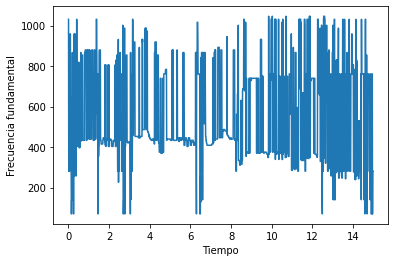
\includegraphics[width=\linewidth]{GLogS.png}
\caption{Estimación con GLogS}
\label{glogs}
\end{minipage}
\hspace{0.5cm}
\begin{minipage}[b]{0.5\linewidth}
\centering
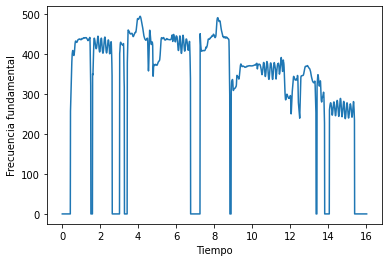
\includegraphics[width=\linewidth]{true.png}
\caption{Estimación esperada}
\label{true}
\end{minipage}
\caption{Comparación entre la estimación esperada y la obtenida }
\label{comparacion1}
\end{figure}

\begin{figure}[h!]
\centering
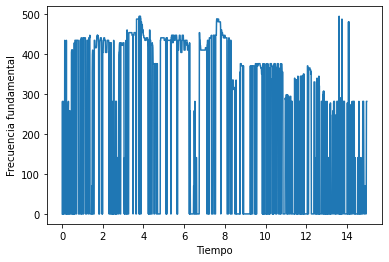
\includegraphics[width=0.5\textwidth]{post.png}
\caption{Estimación luego de establecer un umbral}
\label{post}
\end{figure}


\subsection{Parte 3}
En esta parte se creo un $f_0$ grama con los valores de GLogS y se lo comparo con el espectrograma de la señal. Ambas gráficas se adjuntan en la figura \ref{comparacion}. Con esta comparación se puede entender la presencia de dos bandas de frecuencia en el $f0$ grama, una en el entrono de los 400Hz y otra en el entorno de los 800Hz, era de esperar ya que en el espectrograma hay bandas de frecuencia en esos mismos entornos. En la \ref{f0grama} se ve como claramente la estimación de la frecuencia fundamental no es buena en algunas partes, en el comienzo cerca de los $2s$ hay un buen acercamiento pero en otras partes queda un poco desfasada \footnote{Este desfasaje temporal esta presente en toda la estimación, es muy pequeño por lo que en la parte anterior al comparar entre gráficas diferentes paso desapercibido. Este desfasaje puede ser causado por el largo de las ventanas de la STFT o por el momento en donde se comienza a analizar. De cualquier forma este desfasaje es solo temporal y no es parte de la calidad de la estimación}. A su vez, se puede observar en la figura \ref{soloref} la referencia esta desfasada con lo que se ve en el $f0$ grama, esto era de esperar ya que el $f0$ grama esta construido desde los mismos valores que la estimación es por eso que si se superponen. A su vez el $f0$ grama deja en evidencia que el GlogS también detecta ''energia'' en una segunda banda de frecuencia, en el entorno de los $800Hz$ esta observación es la que permitiría tener una mejor estimación afinando el algoritmo original para que detecte si se esta estimando esa banda o la de mas abajo. Con eso se generaría una estimación de mucha mejor calidad que la obtenida. En otras palabras, queda en evidencia que si hay una detección en $f0$ también hay una detección en $2f0$ y esto se podría haber utilizado para tener una mejor estimación.

\begin{figure}[!h]
\begin{minipage}[b]{0.5\linewidth}
\centering
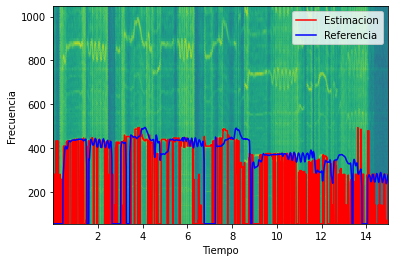
\includegraphics[width=\linewidth]{f0grama.png}
\caption{$f_0$ grama}
\label{f0grama}
\end{minipage}
\hspace{0.5cm}
\begin{minipage}[b]{0.5\linewidth}
\centering
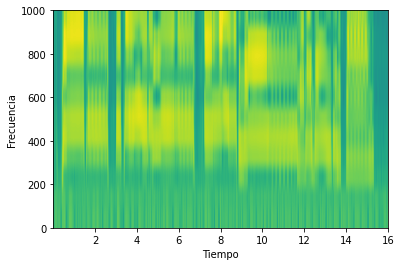
\includegraphics[width=\linewidth]{espectrograma.png}
\caption{Espectrograma}
\label{espect}
\end{minipage}
\caption{$f_0$ grama vs espectrograma}
\label{comparacion}
\end{figure}

\begin{figure}[h!]
\centering
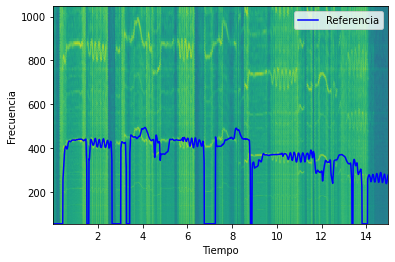
\includegraphics[width=0.5\textwidth]{soloref.png}
\caption{$f_0$ grama solo con la referencia}
\label{soloref}
\end{figure}

\newpage
\section{Ejercicio 3}
Síntesis de la STFT discreta mediante el método de Overlap Add (OLA).
\subsection{Parte 1}
Por definición de DTFT se tiene que
$$X(e^{jw}) = \sum_{n=-\infty}^{+\infty}x[n]e^{-jw}$$
Dado que la funcion $x[n]$ en este caso tiene soporte acotado entre $-M$ y $M-1$ se tiene que su DTFT es
$$W_r(e^{jw}) = \sum_{n=-M}^{M-1}1e^{-jwn}$$
Utilizando el resultado de la serie geométrica donde $N_1 = -M$ y $N_2 = M-1$ $\sum_{n=N_1}^{N_2}\alpha^{k} = \frac{\alpha^{N_1}-\alpha^{N_2+1}}{1-\alpha}$
se tiene que
$$W_r(e^{jw}) = \sum_{n=-M}^{M-1}{(e^{-jw})}^n = \frac{e^{-jw(-M)}-e^{-jw(M)}}{1-e^{-jw}}$$
donde operando se obtiene 
$$    W_r(e^{j\omega}) = \bigg(\frac{1-e^{-j\omega 2M}}{1-e^{-j\omega}}\bigg)e^{j\omega M}$$
\subsection{Parte 2}
La ventana de Hann sigue la siguiente ecuacion
$$w_{Hann}[n]=[0.5 + 0.5cos(\pi n/M)]w_r[n] = 0.5w_r[n] + 0.5cos(\pi n/M)w_r[n]$$
descomponiendo el $cos$ en exponenciales se tiene que
$$w_{Hann}[n] = 0.5w_r[n] + 0.5w_r[n]\frac{1}{2}\big[e^{j(\pi n / M)}+^{-j(\pi n / M)}\big]$$
para calcular la DTFT se utilizara que $x[n]e^{nw_0}=X(e^{jw-w_0})$
de esta manera se obtiene
$$W_{Hann}(e^{j\omega}) = 0.5W_r(e^{j\omega}) +0.25 W_r(e^{j(\omega-\pi/M)})+0.25 W_r(e^{j(\omega+\pi/M)})$$

Sustituyendo por la expresión calculada en la parte anterior se tiene que
$$W_{Hann}(e^{j\omega}) = 0.5\bigg(\frac{1-e^{-j\omega 2M}}{1-e^{-j\omega}}\bigg)e^{j\omega M} + 0.25\bigg(\frac{1-e^{-j(\omega-\pi/M) 2M}}{1-e^{-j(\omega-\pi/M)}}\bigg)e^{j(\omega-\pi/M) M}$$
$$+0.25\bigg(\frac{1-e^{-j(\omega+\pi/M) 2M}}{1-e^{-j(\omega+\pi/M)}}\bigg)e^{j(\omega+\pi/M) M}$$

que operando en las exponenciales se puede expresar como

$$W_{Hann}(e^{j\omega}) = 0.5\bigg(\frac{1-e^{-j\omega 2M}}{1-e^{-j\omega}}\bigg)e^{j\omega M} +
0.25\bigg(\frac{1-e^{-j\omega2M}}{1-e^{-j(\omega-\pi/M)}}\bigg)e^{-j\omega M}+0.25\bigg(\frac{1-e^{-j\omega2M}}{1-e^{-j(\omega+\pi/M)}}\bigg)e^{-j\omega M}$$

\subsection{Parte 3}
En esta parte se realizara la síntesis mediante el método OLA. Para eso se seguirán las ideas presentadas en \cite{RS2}. 
Se comenzara observando que $W_{Hann}(e^{j\omega}) = 0$ para todo $k=1,2,...,M-1$. Esto es dado por el resultado anterior y observando que las raíces de $W_r(e^{jw})$ se dan en múltiplos de $\frac{\pi}{M}$  para $k = 2,4,...,2M-2$ y al correr la ventana $\pm \pi$ estas raíces vuelven a coincidir por lo que se termina anulando en las frecuencias $2 \pi k /M$ para $k = 1,2,...M-1$ como se pedía demostrar. La condición vista en el teórico para la reconstrucción perfecta es que $\sum_{r = -\infty}^{+\infty}w[rR-n]=C$ con $C$ una constante. En este caso $w$ es la ventana de Hann. Se puede ver que 

$$\sum_{r = -\infty}^{+\infty}w[rR-n] = \frac{1}{R}\sum_{k=0}^{R-1}W^*(e^{j(2 \pi K)/R})e^{j(2 \pi K)/R}$$

ya que al ser $\sum_{r = -\infty}^{+\infty}w[rR-n]$ periódica de periodo $R$ se la puede representar como la DFT inversa de $W^*(e^{j(2 \pi K)/R})$ que es la DTFT de $w[-n]$ muestreada en $2 \pi k /R$ en $k = 0,1,2, R-1$. Por lo que para tener la reconstrucción perfecta lo que se necesita es que $|W^*(e^{j(2 \pi K)/R})| = |W(e^{j(2 \pi K)/R})| = 0$ $\forall k = 1,...,R-1$. De esta manera $C = \frac{W(e^{j0})}{R}$.

En el caso de la ventana Hann, ya se explico que hay un subset de 0s en $\frac{2\pi k}{M}$, como lo que se quiere es que $\frac{2\pi k}{M} = \frac{2\pi k}{R}$ se tiene que si se elige $R=M$ se cumple la condición o que si $M/2$ es un entero se puede tomar $R = \frac{M}{2}$.

\subsection{Parte 4}
Del teórico se sabe que $W(e^{jw}) = \sum_{m=-\infty}^{+\infty}w[m]e^{-jwm}$
como se quiere evaluar en $w=0$ se quiere encontrar
$W(e^{j0}) = \sum_{m=-\infty}^{+\infty}w[m]$. 
En este caso se tiene que 

$$W(e^{j0}) = \sum_{m=-M}^{M-1}(0.5+0.5cos(\pi m / M)) \sum_{m=-M}^{M-1}0.5+0.5\sum_{m=-M}^{M-1}\frac{1}{2}\bigg(e^{j\pi /M}^m + e^{-j\pi /M}^m  \bigg)$$

donde la primer sumatoria tiene como resultado $0.5(M-1-(-M)) = M$ y la segunda se resuelve con la serie geométrica utilizada anteriormente. $\sum_{m=-M}^{M-1}e^{j\pi /M}^m = \frac{e^{(j\pi /M)(-M)} - e^{(j\pi /M)(M)}}{1-e^{j\pi /M}} = \frac{-1-(-1)}{1-e^{j\pi /M}} = 0$ y $\sum_{m=-M}^{M-1}e^{-j\pi /M}^m = \frac{e^{-(j\pi /M)(-M)} - e^{(-j\pi /M)M}}{1-e^{-j\pi /M}} = \frac{-1-(-1)}{1-e^{j\pi /M}} = 0$
por lo que termina siendo 

$$W(e^{j0}) = M$$

y utilizando el resultado de la parte anterior para la reconstrucción perfecta se tiene que 
$$C = \frac{W(e^{j0})}{R} = \frac{M}{R}$$

\section{Ejercicio 4}
Implementación del Phase-Vocoder.
\subsection{Parte 1}
Como fue visto en el ejercicio anterior para tener reconstrucción perfecta al utilizar una ventana Hann se necesita que $R = M$ o que en su defecto $R = M/2$ mientras ese numero sea entero. Para escribir los algoritmos no se usa el parámetro $M$ si no que se utiliza $L$ que es el largo de la ventana. En este caso, lo que se tiene es que $M = L/2$ ya que el largo de la ventana es $2M$. Dado que hay que elegir una de las opciones, se opta por elegir $L = 2048$ y $R = L / 2$ que implica $R=M$. Por el ejercicio anterior también se sabe que $C = W(e^{j0})/R$, en este caso $C=1$. Esto se verifica experimentalmente con los resultados de la gráfica de la figura \ref{ola} donde se puede ver la ventana de análisis y luego el resultado de hacer Overlap Add generando una constante.

\begin{figure}[h!]
\centering
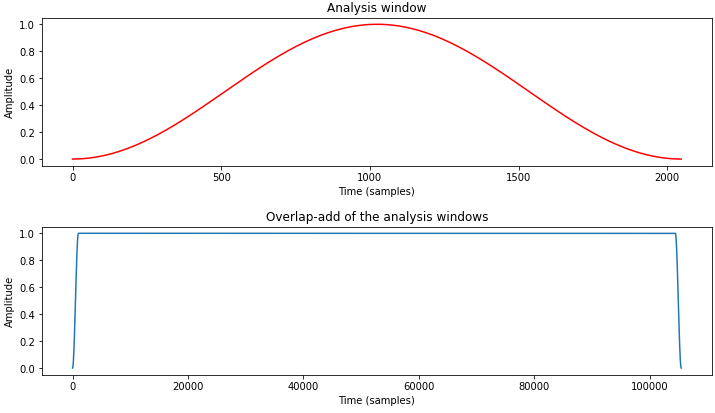
\includegraphics[width=0.8\textwidth]{resultadola.png}
\caption{Verificación experimental de la elección de L y R}
\label{ola}
\end{figure}

Luego de realizar el análisis y la síntesis utilizando el mismo $R$ en ambos casos, al haber respetado la condición explicada anteriormente se obtiene la misma señal del comienzo. Esto era esperable pues se esta realizando una reconstrucción perfecta. Los resultados se presentan en forma de gráfica en la figura \ref{resuas} donde se aprecia que la señal original y la que se obtiene luego del análisis y síntesis son exactamente iguales. Esto también se comprobó auditivamente. 

\begin{figure}[h!]
\centering
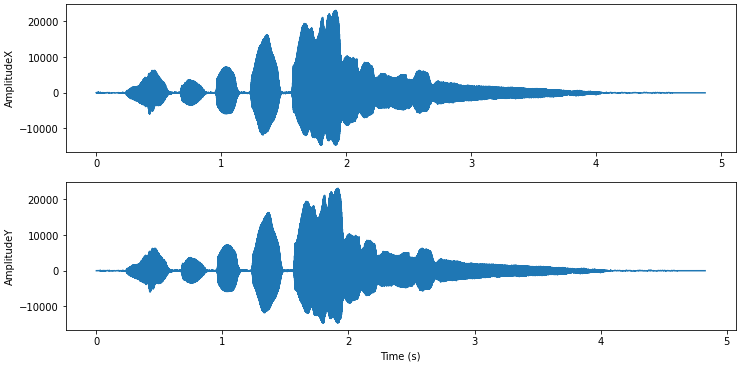
\includegraphics[width=0.8\textwidth]{resuas.png}
\caption{Señal original arriba y señal luego del análisis y síntesis con el mismo R abajo}
\label{resuas}
\end{figure}

\subsection{Parte 2}
En esta parte se introducirán cambios en la escala temporal cambiando el $R$ de la síntesis. Para alargar la escala temporal se tomara un $R_S$ mayor que el de antes, específicamente el doble lo que generara que se duplique la escala temporal. Esto se puede apreciar en la figura \ref{doble} donde la gráfica que tiene en el eje vertical la etiqueta de AmplitudY corresponde a la procesada. Al cambiar la escala temporal se perciben cambios de manera auditiva. Entre ellos la introducción de artefactos de estilo ''roboticos'' y algunos ''rings'' en diversas partes del audio. Esto es causado por el solapamiento de tramas cuya fase no es coherente. Es decir hubo un salto temporal pero la fase se mantuvo igual. Dado que la ventana es lo suficientemente grande, se sigue escuchando la altura de la señal.

\begin{figure}[h!]
\centering
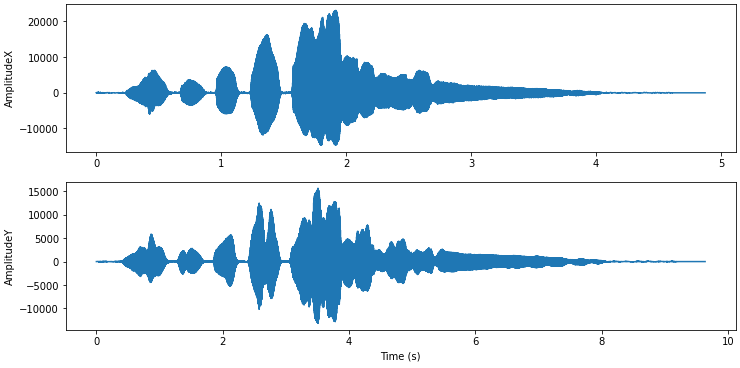
\includegraphics[width=0.8\textwidth]{doble.png}
\caption{Análisis y síntesis con mismo $R_s = 2R_a$}
\label{doble}
\end{figure}

Luego se probo reduciendo el $R_s$ a la mitad para lograr reducir la escala temporal también a la mitad. Esto se puede apreciar en la figura \ref{mitad} donde la gráfica que tiene en el eje vertical la etiqueta de AmplitudY corresponde a la procesada. En este caso la primer diferencia se ve en el cambio de la escala temporal como era de esperar y auditivamente por mas de que se sigue escuchando la altura de la señal, se escuchan algunos defectos causados por las incoherencias de fase. 

\begin{figure}[h!]
\centering
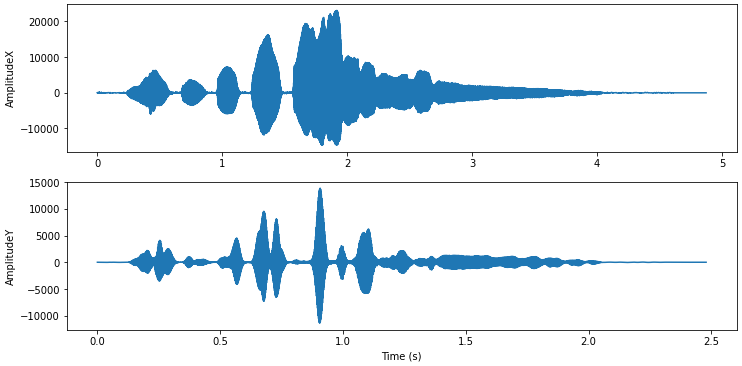
\includegraphics[width=0.8\textwidth]{mitad.png}
\caption{Análisis y síntesis con mismo $R_s = R_a/2$}
\label{mitad}
\end{figure}

\subsection{Parte 3}
Para revertir las consecuencias de utilizar diferentes tamaños de $R$ en el análisis y síntesis se realiza el desdoblamiento de fase. Este intentara arreglar las inconsistencias de fase ignoradas hasta el momento. Para realizarlo se siguieron los procedimientos sugeridos en \cite{PV}. En un principio se considero el análisis y la síntesis con las funciones realizadas en clase, sin embargo el resultado no fue satisfactorio, auditivamente se escuchaban ruidos un tanto roboticos y como se muestra en la comparación de la figura \ref{pvmal} en el espectro la fase no se había arreglado completamente. 

\begin{figure}[!h]
\begin{minipage}[b]{0.5\linewidth}
\centering
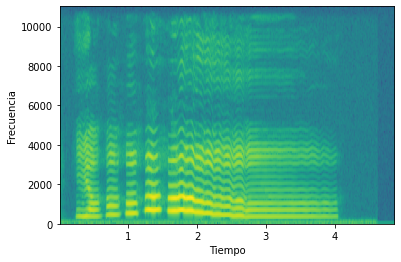
\includegraphics[width=\linewidth]{original.png}
\caption{Espectrograma original}
\label{original}
\end{minipage}
\hspace{0.5cm}
\begin{minipage}[b]{0.5\linewidth}
\centering
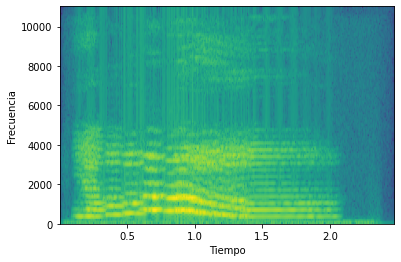
\includegraphics[width=\linewidth]{pvmal.png}
\caption{Luego del desdoblamiento de fase}
\label{espect}
\end{minipage}
\caption{Comparación de espectrogramas antes y después del desdoblamiento de fase}
\label{pvmal}
\end{figure}

Luego de inspección del código y la letra y se constato que el código realizado en la clase no realiza un enventanamiento en la síntesis, por lo que se agrego un enventanamiento con la misma ventana que en el análisis, en este caso el resultado si fue satisfactorio tanto auditivamente como visualmente a través de los espectros como se muestra en la figura \ref{pvbien}. Con este error se puedo apreciar la gran influencia que tiene el enventanamiento en la síntesis para obtener un buen resultado. La razón detrás por la cual esto mejora el resultado es que el multiplicar por la ventana a la señal reconstruida asegura que no se escapen discontinuidades de fase al principio o al final de un frame. Vale aclarar que al enventanar también se debe realizar el escalamiento correspondiente, en este caso es dado por la ventana de análisis y la ventana de suavizado que se aplico en síntesis. 

\begin{figure}[!h]
\begin{minipage}[b]{0.5\linewidth}
\centering
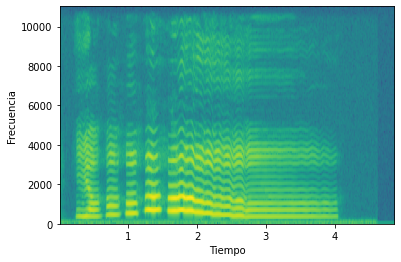
\includegraphics[width=\linewidth]{original.png}
\caption{Espectrograma original}
\label{original}
\end{minipage}
\hspace{0.5cm}
\begin{minipage}[b]{0.5\linewidth}
\centering
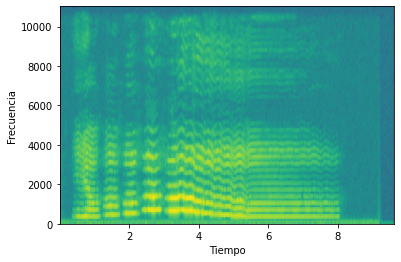
\includegraphics[width=\linewidth]{pvbien.png}
\caption{Luego del desdoblamiento de fase}
\label{espect}
\end{minipage}
\caption{Comparación de espectrogramas antes y después del desdoblamiento de fase}
\label{pvbien}
\end{figure}

\newpage
\subsection{Parte 4}
En esta parte se utilizo el phase vocoder con el desdoblamiento de fase correcto para realizar pitch shifting. Auditivamente el resultado fue satisfactorio ya que se nota un cambio de altura en la señal pero con la misma base temporal. En este caso se mantiene la escala temporal pero si se cambia el contenido en frecuencia, especialmente se puede observar como el contenido en frecuencia es el mismo pero los componentes están mas espaciados. Esto se puede ver en la comparación de espectrogramas de la figura \ref{ps} 

\begin{figure}[!h]
\begin{minipage}[b]{0.5\linewidth}
\centering
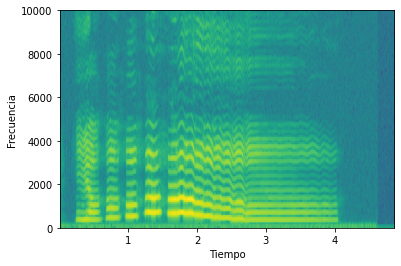
\includegraphics[width=\linewidth]{original2.png}
\caption{Espectrograma original}
\label{original}
\end{minipage}
\hspace{0.5cm}
\begin{minipage}[b]{0.5\linewidth}
\centering
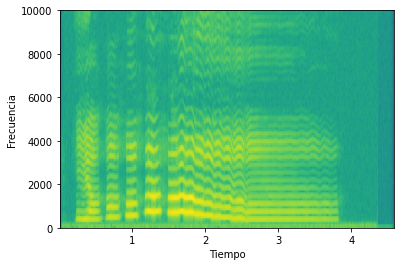
\includegraphics[width=\linewidth]{pitchshift.png}
\caption{Luego del pitch shifting}
\label{espect}
\end{minipage}
\caption{Comparación de espectrogramas luego del pitch shifting}
\label{ps}
\end{figure}




\newpage
\begin{thebibliography}{100} % 100 is a random guess of the total number of
%references
\addtolength{\leftmargin}{0.2in} % sets up alignment with the following line.
\setlength{\itemindent}{-0.2in}
\bibitem[RS1]{RS1}Rabiner, L. R. (2011). Pitch Period Estimation (Pitch Detection). In R. W. Schafer (Ed.), Theory and applications of Digital Speech Processing (First ed., pp. 623–625). Pearson.
\bibitem[RS2]{RS2} Rabiner, L. R. (2011a). Frequency-domain representations. In R. W. Schafer (Ed.), Theory and applications of Digital Speech Processing (First ed., pp. 322–329). Pearson.
\bibitem[PV]{PV} de Götzen, A., Bernardini, N., & Arfib, D. (2000, December). Traditional implementations of a phase-vocoder: The tricks of the trade. Proceedings of the COST G-6 Conference on digital audio effects, Verona, Italy.
\bibitem[OF10]{of10} [Analisis de Fourier de tiempo corto], [Martín Rocamora], Proyecto OpenFING, [https://open.fing.edu.uy/courses/audiodsp/10], publicado bajo una licencia CC By NC ND.
\bibitem[OF11]{of11}[Representaciones tiempo-frecuencia multi-resolución], [Martín Rocamora], Proyecto OpenFING, [https://open.fing.edu.uy/courses/audiodsp/11], publicado bajo una licencia CC By NC ND.
\bibitem[OF12]{of12}[Análisis y síntesis con la STFT], [Martín Rocamora], Proyecto OpenFING, [https://open.fing.edu.uy/courses/audiodsp/12], publicado bajo una licencia CC By NC ND.
\bibitem[OF13]{of13}[Procesamiento tiempo-frecuencia], [Martín Rocamora], Proyecto OpenFING, [https://open.fing.edu.uy/courses/audiodsp/13], publicado bajo una licencia CC By NC ND.

\bibitem[OF14]{of14}[Phase Vocoder], [Martín Rocamora], Proyecto OpenFING, [https://open.fing.edu.uy/courses/audiodsp/14], publicado bajo una licencia CC By NC ND.
\end{thebibliography}



\end{document}